\chapter{Confronto}
\section{Scansione delle vulnerabilità}
Il database di entrambi gli strumenti è un aspetto cruciale per la qualità e l'accuratezza delle analisi di vulnerabilità. Trivy e Snyk utilizzano database di vulnerabilità differenti, che influenzano la loro capacità di identificare e classificare le vulnerabilità.
\subsection{Vulnerabilità nella Supply Chain}
La struttura "a strati" dei container Docker permette un'enorme flessibilità dal punto di vista dello sviluppo e della distribuzione delle applicazioni, ma introduce anche una serie di nuove sfide per la sicurezza. Le immagini Docker sono costruite a partire da altre immagini che possono contenere una vasta gamma di pacchetti e librerie, ognuno dei quali può essere vulnerabile a una serie di minacce.

Sulla base di ciò, possono quindi nascere due nuove classificazioni di vulnerabilità:

\begin{itemize}
   \item \textbf{Vulnerabilità ereditate}: vulnerabilità presenti nella base image utilizzata per costruire l'immagine Docker.
   \item \textbf{Vulnerabilità installate}: vulnerabilità presenti nei pacchetti e nelle librerie installate dall'utente nell'immagine Docker.
\end{itemize}
È quindi necessario categorizzare le vulnerabilità in base alla loro origine, perché il modo in cui esse devono essere affrontate è differente.
\begin{itemize}
   \item Le vulnerabilità ereditate richiedono una modifica della base image. Per risolverle, potrebbe essere necessario aggiornare la base image, o sostituirla con una versione alternativa. Quest'ultimo processo può essere complesso e dispendioso, in quanto può richiedere la modifica della pipeline di sviluppo e la verifica della compatibilità tra l'applicazione esistente e la nuova base image.
   \item Le vulnerabilità installate possono essere corrette più facilmente, tipicamente aggiornando i pacchetti e le librerie installate all'interno dell'immagine. Questo processo è generalmente più semplice e meno dispendioso rispetto alla correzione delle vulnerabilità ereditate.
\end{itemize}


In questa prima parte di testing, si è voluto valutare la capacità di Trivy e Snyk di identificare e classificare le vulnerabilità presenti in immagini Docker altamente utilizzate. Per fare ciò, si è utilizzato un campione di immagini di container, e si è confrontato il risultato delle scansioni di Trivy e Snyk. I risultati di questi test sono stati valutati in base alla precisione e alla completezza delle informazioni fornite da Trivy e Snyk.

Le immagini Docker sottoposte a scansione sono state selezionate in base alla loro popolarità e alla loro rilevanza nel panorama delle applicazioni e dei servizi cloud. In particolare, si è scelto di testare le seguenti immagini:
\begin{itemize}
   \item\textbf{nginx}: uno dei principali server web e reverse proxy.
   \item\textbf{mongo}: database NoSQL flessibile e scalabile basato su MongoDB.
   \item\textbf{wordpress}: piattaforma di blogging e CMS.
   \item\textbf{alpine}: una delle immagini di container più leggere e minimali, basata su Alpine Linux È ampiamente usata come base per altre immagini di container.
   \item\textbf{node}: ambiente di esecuzione per JavaScript basato su Chrome V8.
\end{itemize}
Inoltre, si è voluto testare due tipi di versioni per ogni immagine: la versione più recente, e una versione più datata.
Nella tabella \ref{tab:scan_results} sono riportati i risultati ottenuti da entrambi i tool per ciascuna immagine testata.
\begin{table}[H]
   \centering
   \begin{tabularx}{\textwidth}{|l|l|X|X|X|X|X|X|X|X|}
      \hline
      \textbf{Immagine}          & \textbf{Vers.} & \multicolumn{4}{c|}{\textbf{Snyk}} & \multicolumn{4}{c|}{\textbf{Trivy}}                                                                                              \\ \cline{3-10}
                                 &                & \textbf{Crit.}                     & \textbf{High}                       & \textbf{Mid} & \textbf{Low} & \textbf{Crit.} & \textbf{High} & \textbf{Mid} & \textbf{Low} \\ \hline
      \multirow{2}{*}{nginx}     & latest         & 1                                  & 6                                   & 3            & 78           & 2              & 16            & 34           & 83           \\ \cline{2-10}
                                 & v1.23.0        & 10                                 & 39                                  & 73           & 111          & 16             & 80            & 139          & 115          \\ \hline
      \multirow{2}{*}{mongo}     & latest         & 0                                  & 0                                   & 1            & 12           & 0              & 0             & 1            & 21           \\ \cline{2-10}
                                 & v4.4.3         & 0                                  & 7                                   & 88           & 69           & 0              & 13            & 195          & 105          \\ \hline
      \multirow{2}{*}{wordpress} & latest         & 1                                  & 1                                   & 3            & 150          & 3              & 50            & 143          & 326          \\ \cline{2-10}
                                 & v6.0.0         & 23                                 & 66                                  & 142          & 228          & 49             & 340           & 509          & 547          \\ \hline
      \multirow{2}{*}{alpine}    & latest         & 0                                  & 0                                   & 0            & 0            & 0              & 0             & 0            & 0            \\ \cline{2-10}
                                 & v3.11          & 1                                  & 0                                   & 0            & 0            & 1              & 0             & 0            & 0            \\ \hline
      \multirow{2}{*}{node}      & latest         & 1                                  & 4                                   & 3            & 160          & 5              & 73            & 246          & 481          \\ \cline{2-10}
                                 & v16.0.0        & 48                                 & 183                                 & 275          & 390          & 140            & 970           & 1353         & 1417         \\ \hline
   \end{tabularx}
   \caption{Risultati delle scansioni di Snyk e Trivy per ciascuna immagine testata.}
   \label{tab:scan_results}
\end{table}
\subsection{Risultati delle scansioni}
Dai risultati ottenuti, si evincono le seguenti considerazioni:
\subsubsection{Numero di vulnerabilità rilevate}
Trivy generalmente avvisa di un numero maggiore di vulnerabilità rispetto a Snyk. Questo è particolarmente evidente per le versioni più datate delle immagini, dove Trivy rileva un numero significativamente maggiore di vulnerabilità. Da solo, il mero numero di vulnerabilità rilevate non è un indicatore della qualità o dell'accuratezza delle scansioni, per via della presenza di eventuali falsi positivi o di vulnerabilità non rilevate. Dopo un'ispezione manuale a campione, è stato però visto che la quasi totalità delle vulnerabilità era effettivamente tale, seppure la loro gravità fosse praticamente trascurabile. I rari casi si sono sempre limitati ad estremamente sporadici.


\subsubsection{Differenza nella classificazione delle stesse vulnerabilità}
Gli strumenti hanno riportato, in molti casi, una differenza nelle classificazioni delle stesse vulnerabilità. Questo è dovuto alla differenza di valutazione delle vulnerabilità da parte dei database utilizzati. In particolare, Snyk tende a classificare le vulnerabilità in modo più conservativo, assegnando un numero inferiore di vulnerabilità di livello critico e alto rispetto a Trivy. Ad esempio, per l'immagine \texttt{nginx:latest}, entrambi i tool hanno rilevato correttamente la vulnerabilità CVE-2023-6879, relativa ad un buffer overflow presente nella libreria \texttt{AOMedia}, ma mentre Trivy ha classificato la vulnerabilità come di livello critico, Snyk ha classificato la stessa come di livello basso. Questa differenza è dovuta alle sorgenti di informazioni di valutazione utilizzate dai due tool:
\begin{itemize}
   \item Trivy utilizza la classificazione NVD, che è nota per essere meno conservativa nella classificazione delle vulnerabilità, assegnando quindi un numero maggiore di vulnerabilità di livello critico o alto.
   \item Snyk invece assegna la categoria in base a tre elementi di valutazione:
         \begin{itemize}
            \item L'analisi interna condotta dal team di Snyk.
            \item Una valutazione della gravità fornita dal team di sicurezza del manutentore della distribuzione Linux.
            \item La gravità della vulnerabilità secondo il database NVD.
         \end{itemize}
\end{itemize}
Visitando infatti il sito web \texttt{security-tracker.debian.org}, è possibile osservare che la vulnerabilità CVE-2023-6879 è stata classificata come di livello basso dal team di sicurezza di Debian, e questo ha influenzato in modo predominante la classificazione di Snyk.
\subsubsection{Confermata di presenza di vulnerabilità ereditate dalla Base Image}
È stata inoltre confermata la presenza di vulnerabilità "ereditate" dalla Base Image: ad esempio, l'unica vulnerabilità che Snyk rileva come critica nell'ultima versione delle immagini \texttt{nginx, wordpress, node} è la stessa vulnerabilità CVE-2023-45853. Questa vulnerabilità è attualmente presente nel sistema Debian e relativa alla libreria \texttt{zlib}, ed è stata quindi ereditata dalle immagini Docker che utilizzano Debian come base image.
Trivy riporta anch'esso che la vulnerabilità è critica, ma anche che essa ha uno stato \texttt{will\_not\_fix}. Ciò indica che tale vulnerabilità è conosciuta, ma al momento non ci sono piani per una correzione. Snyk non riporta invece tale informazione.


\subsection{Formati di output}
Entrambi gli strumenti offrono la possibilità di generare report in vari formati per permetterne, ad esempio, l'integrazione diretta con altri strumenti.
\subsubsection{Trivy}
Il formato di output di default di Trivy è il formato tabulare (Figura \ref{fig:trivy_output_fmt}), che fornisce un report strutturato e facilmente leggibile delle vulnerabilità rilevate.
\begin{figure}[H]
   \centering
   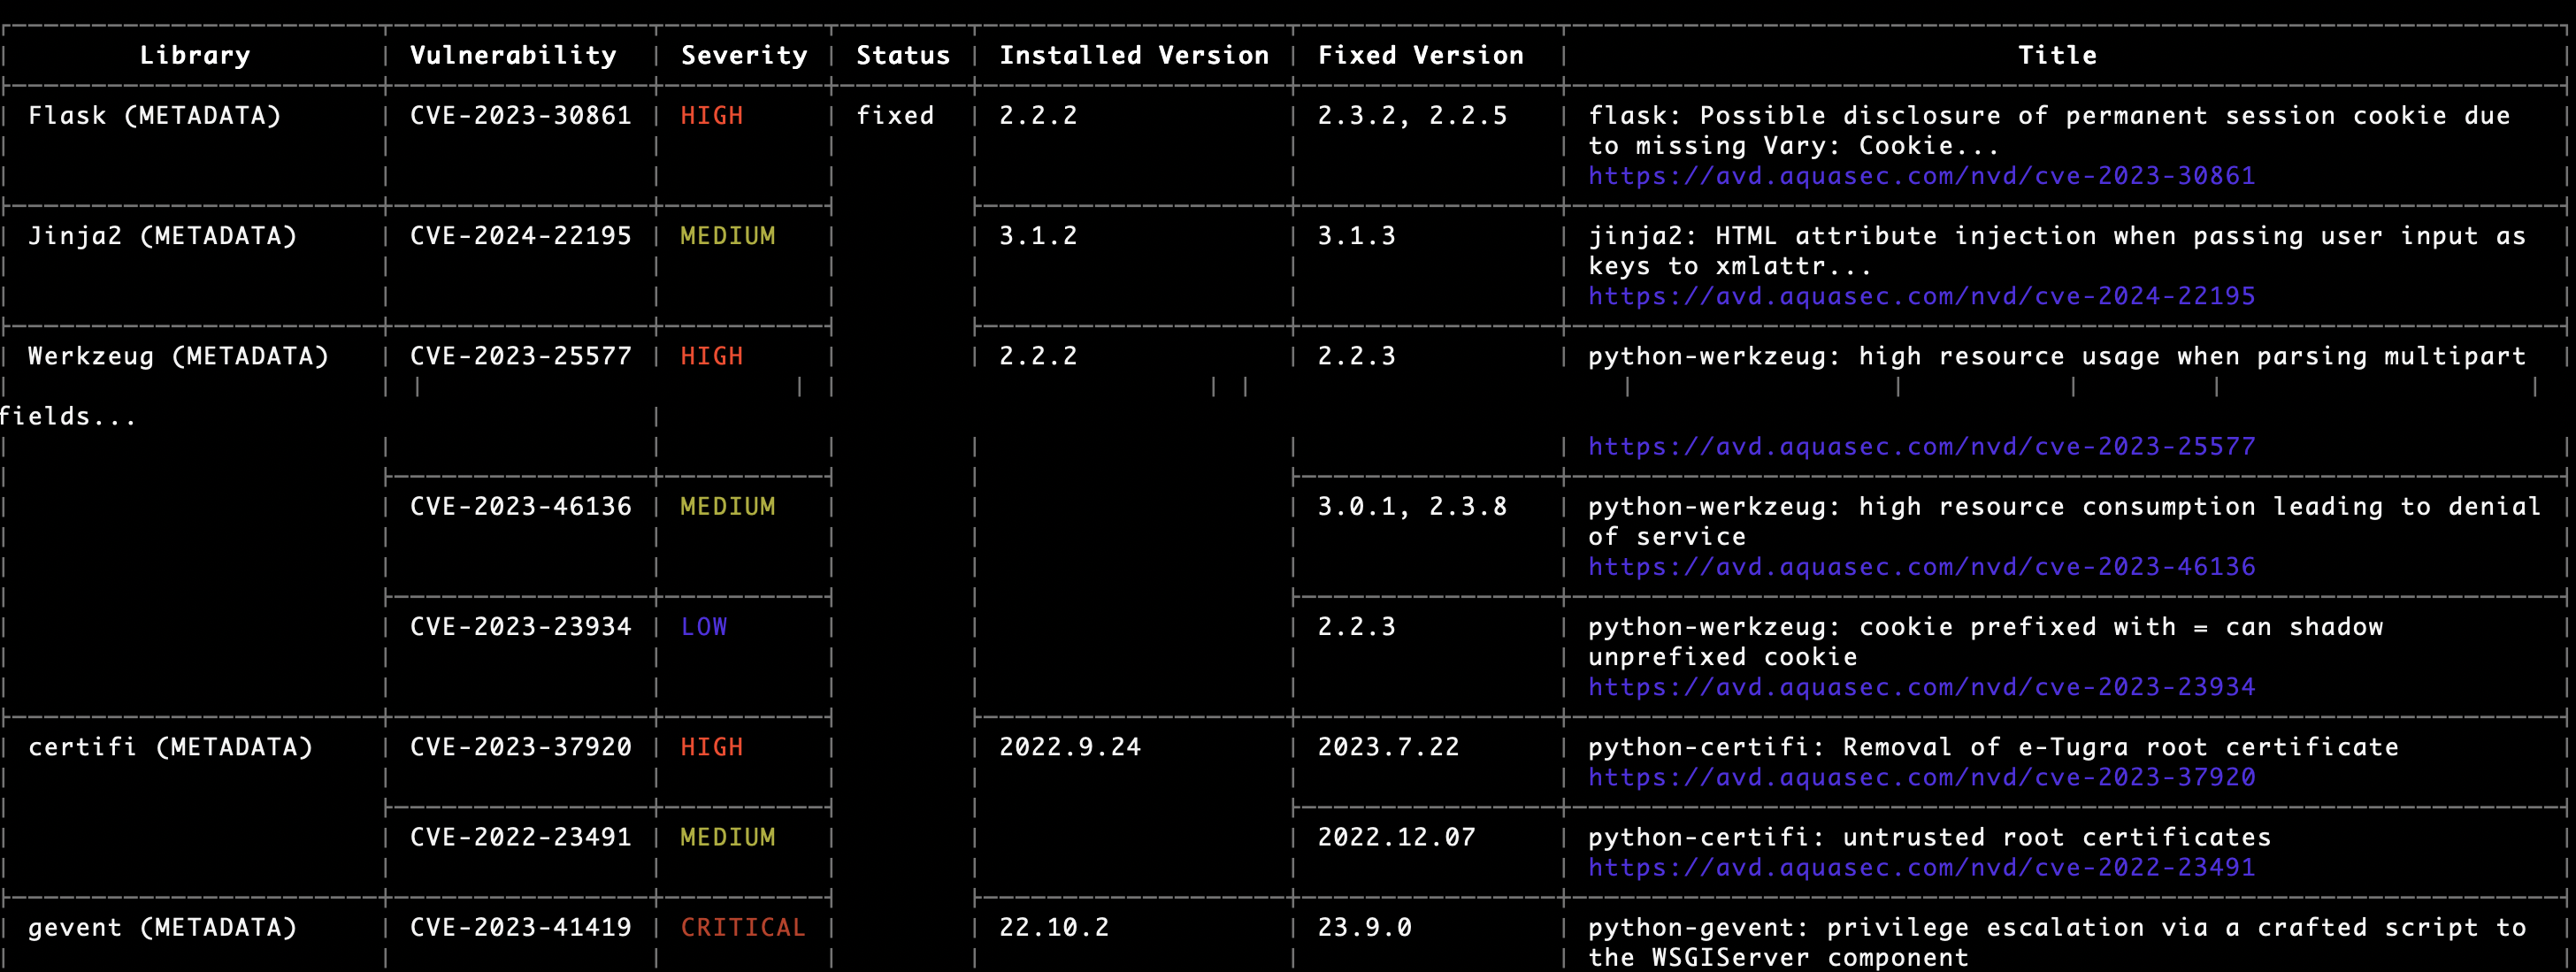
\includegraphics[width=1\textwidth]{immagini/capitolo2/trivy_output_fmt.png}
   \caption{Formato di output di default di Trivy}
   \label{fig:trivy_output_fmt}
\end{figure}
Inoltre, Trivy permette di generare report nei seguenti formati:
\begin{itemize}
   \item \textbf{JSON}
   \item \textbf{JUnit XML}: un formato di output standard per i risultati dei test.
   \item \textbf{Sarif}: un formato di output standard per gli strumenti di analisi statica del codice.
   \item \textbf{Personalizzato}: se i formati predefiniti non soddisfano le esigenze, è possibile specificare un formato di output completamente personalizzato.
\end{itemize}

\subsubsection{Snyk}
Nel formato di default, Snyk restituisce un report in formato "lista" (Figura \ref{fig:snyk_output_fmt}), con l'elenco di tutte le vulnerabilità rilevate.
\begin{figure}[H]
   \centering
   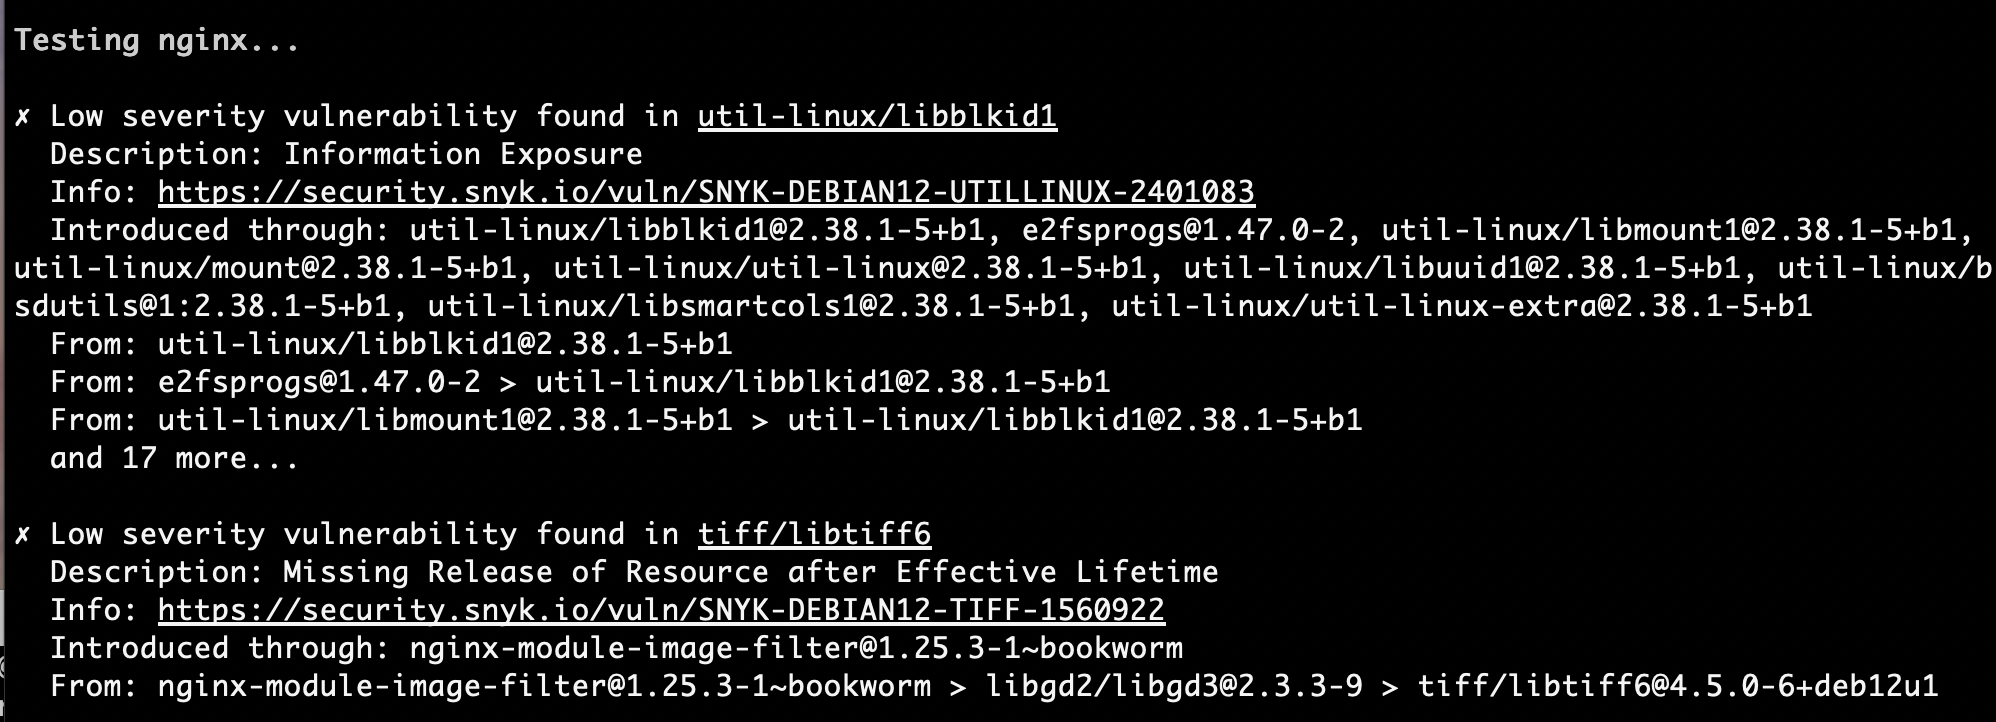
\includegraphics[width=1\textwidth]{immagini/capitolo2/snyk_output_fmt.png}
   \caption{Formato di output di default di Snyk}
   \label{fig:snyk_output_fmt}
\end{figure}

Inoltre, vengono mostrati anche:
\begin{itemize}
   \item Il numero totale di vulnerabilità rilevate.
   \item \textbf{Consigli per la base image}: Snyk propone una base image successiva o alternativa, per notificare l'utente che aggiornando la base image alcune delle vulnerabilità rilevate siano state risolte (Figura \ref{fig:snyk_altn_imgs}).
         \begin{figure}[H]
            \centering
            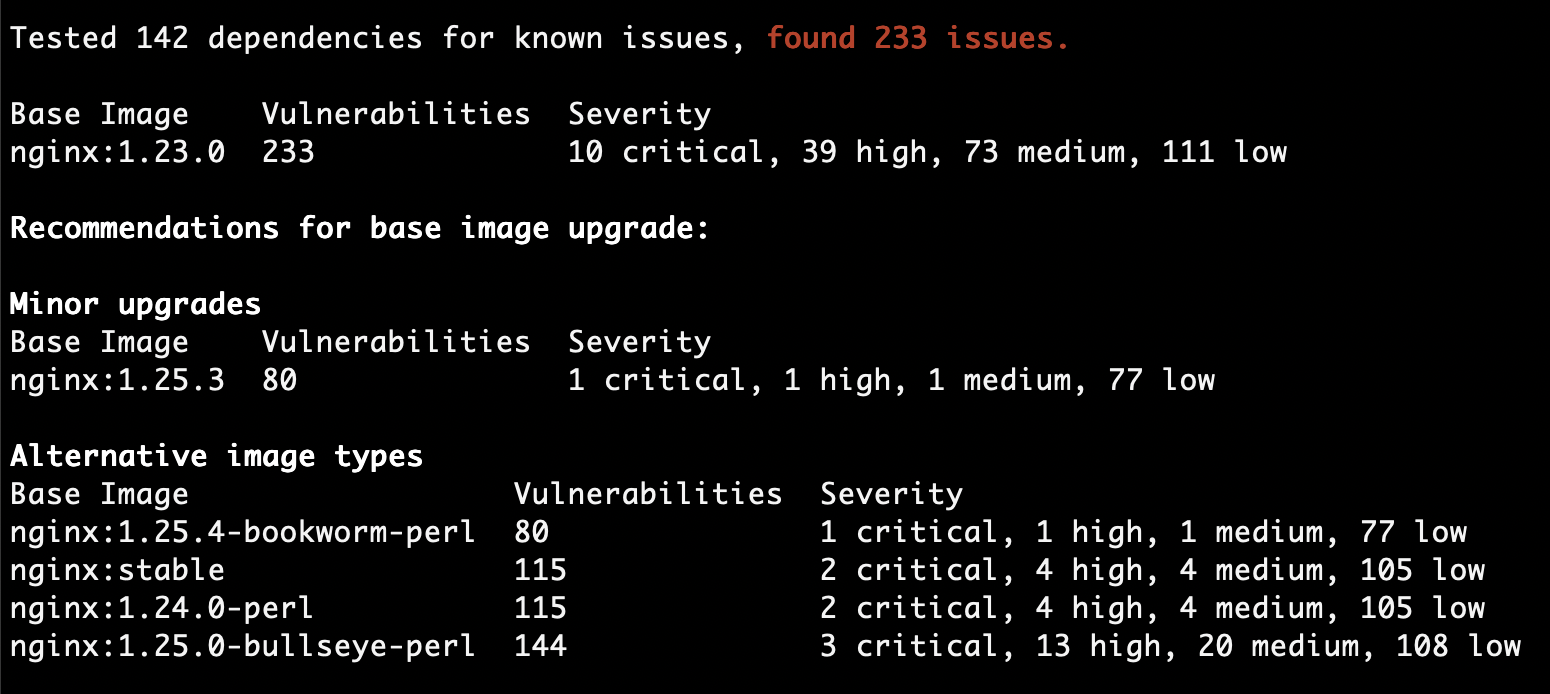
\includegraphics[width=1\textwidth]{immagini/capitolo2/snyk_altn_images.png}
            \caption{Snyk: Consigli per una base image alternativa.}
            \label{fig:snyk_altn_imgs}
         \end{figure}
\end{itemize}

Inoltre, Snyk permette di generare report nei seguenti formati:
\begin{itemize}
   \item\textbf{JSON}
   \item\textbf{SARIF}
\end{itemize}

Differentemente da Trivy, Snyk non permette di generare report in formati tabellari o personalizzati.

\section{Scansione di configurazioni IaC}
Un'altra funzionalità offerta da entrambi i tool è relativa alla scansione di configurazioni IaC, al fine di rilevare problemi di sicurezza o cattive pratiche di configurazione. Per testare tale funzionalità, si è utilizzato un campione di file di configurazione di Terraform, appropriatamente configurato con una vulnerabilità di esempio nota e ben documentata. Il codice in questione è il seguente:
\begin{lstlisting}
   provider "aws" {
      region = "us-east-1"
    }
    
    resource "aws_s3_bucket" "bucket_insecure" {
      bucket = "my-insecure-bucket"
      acl    = "public-read"
    
      tags = {
        Name        = "Insecure Bucket"
        Environment = "Test"
      }
    }
    
\end{lstlisting}


La vulnerabilità in questione è rappresentata dalla configurazione errata delle politiche di accesso su un bucket S3 di AWS, il quale è stato impostato per permettere l'accesso in lettura al pubblico di tutto il bucket (public-read). Tale configurazione espone i dati contenuti nel bucket a potenziali accessi non autorizzati, rappresentando un rischio significativo per la sicurezza dei dati.
Eseguendo la scansione del codice soprastante con entrambi gli strumenti, sono state rilevate le seguenti vulnerabilità:

\begin{center}
   \begin{tabularx}{0.8\textwidth}{|X|X|X|X|X|}
      \hline
      \textbf{Strumento} & \textbf{Critical} & \textbf{High} & \textbf{Medium} & \textbf{Low} \\
      \hline
      Snyk               & 0                 & 0             & 1               & 3            \\
      \hline
      Trivy              & 0                 & 7             & 1               & 2            \\
      \hline
   \end{tabularx}
\end{center}

Tra le vulnerabilità rilevate, in entrambi i casi è stata rilevata la vulnerabilità desiderata. Su Snyk, la vulnerabilità è stata classificata come l'unica di livello medio. Trivy, invece, ha classificato la vulnerabilità come di livello alto. Questa differenza è dovuta alla diversa classificazione delle vulnerabilità da parte dei database utilizzati, come già discusso in precedenza.
Le altre vulnerabilità di livello alto rilevate da Trivy sono state:
\begin{itemize}
   \item \textbf{Quattro vulnerabilità} molto simili tra loro, relative alla mancanza di ACLs sul bucket S3. (No public access block so not blocking public acls)
   \item \textbf{Bucket does not have encryption enabled:} Questa vulnerabilità è stata rilevata in quanto il bucket S3 non ha configurato correttamente la cifratura dei dati.
   \item \textbf{Bucket does not encrypt data with a customer managed key:} Questa vulnerabilità è stata rilevata in quanto il bucket S3 non ha una configurazione per la cifratura dei dati con una chiave gestita dal cliente.

\end{itemize}

\begin{figure}[H]
   \centering
   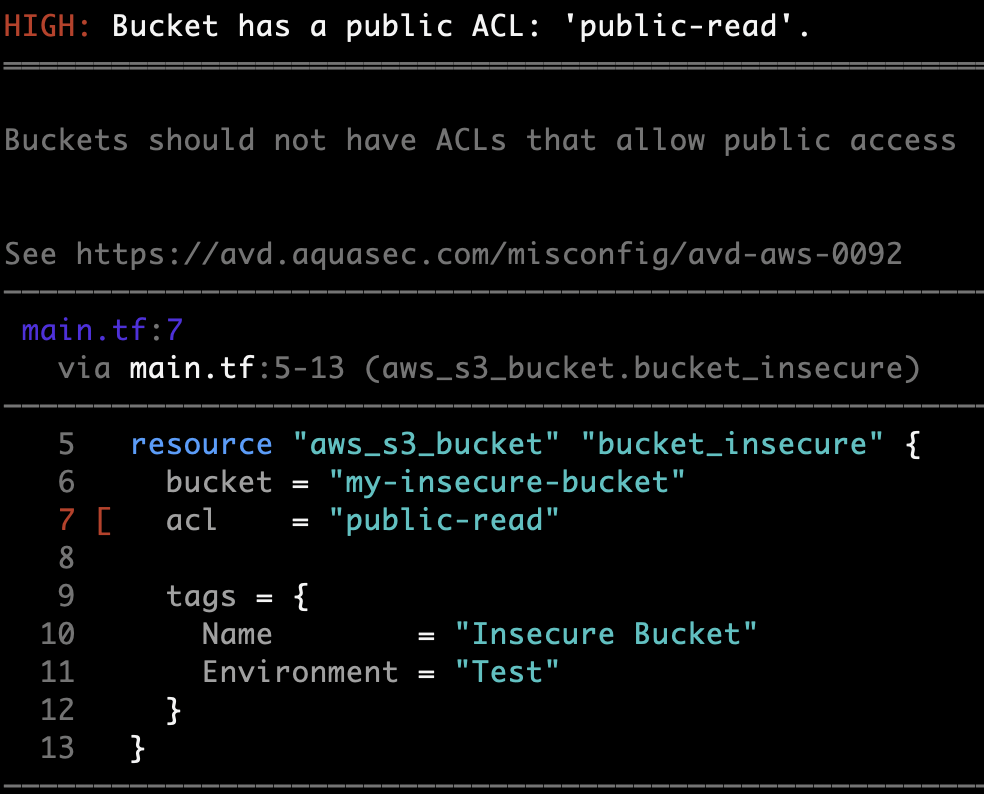
\includegraphics[width=0.6\textwidth]{immagini/capitolo2/trivy_iac.png}
   \caption{Trivy: corretto riconoscimento della vulnerabilità public-read}
   \label{fig:trivy_iac}
\end{figure}

Questi errori non sono stati rilevati da Snyk, che però ha rilevato due possibili vulnerabilità di livello basso non rilevate invece da Trivy:
\begin{itemize}
   \item \textbf{S3 bucket MFA delete control disabled:} Questa vulnerabilità è stata rilevata in quanto nel bucket S3 non è stato configurato correttamente il controllo Multi-Factor Authentication per prevenire la cancellazione dei dati.
   \item \textbf{S3 server access logging is disabled:} Questa vulnerabilità è stata rilevata in quanto il bucket S3 non ha configurato correttamente il logging degli accessi al server.

\end{itemize}


\section{Funzionalità uniche per ogni prodotto}
Durante il testing, sono state rilevate inoltre le funzionalità presenti in uno dei due strumenti, ma non nell'altro. Le funzionalità sono descritte di seguito. Essendo uniche per ogni prodotto, non è stato possibile confrontarle direttamente.

\subsection{Snyk: Monitoraggio Continuo}
Snyk offre un monitoraggio continuo delle applicazioni e delle dipendenze, inviando notifiche in tempo reale in caso di nuove vulnerabilità che influenzano il codice già in uso. Questo assicura che i team possano reagire rapidamente a nuove minacce. Durante il testing, è stato possibile osservare il funzionamento di questa funzione, avendo ricevuto e-mail contenenti nuove vulnerabilità pubblicate solamente giorni prima, come riportato in Figura \ref{fig:snyk_email}.

\begin{figure}[H]
   \centering
   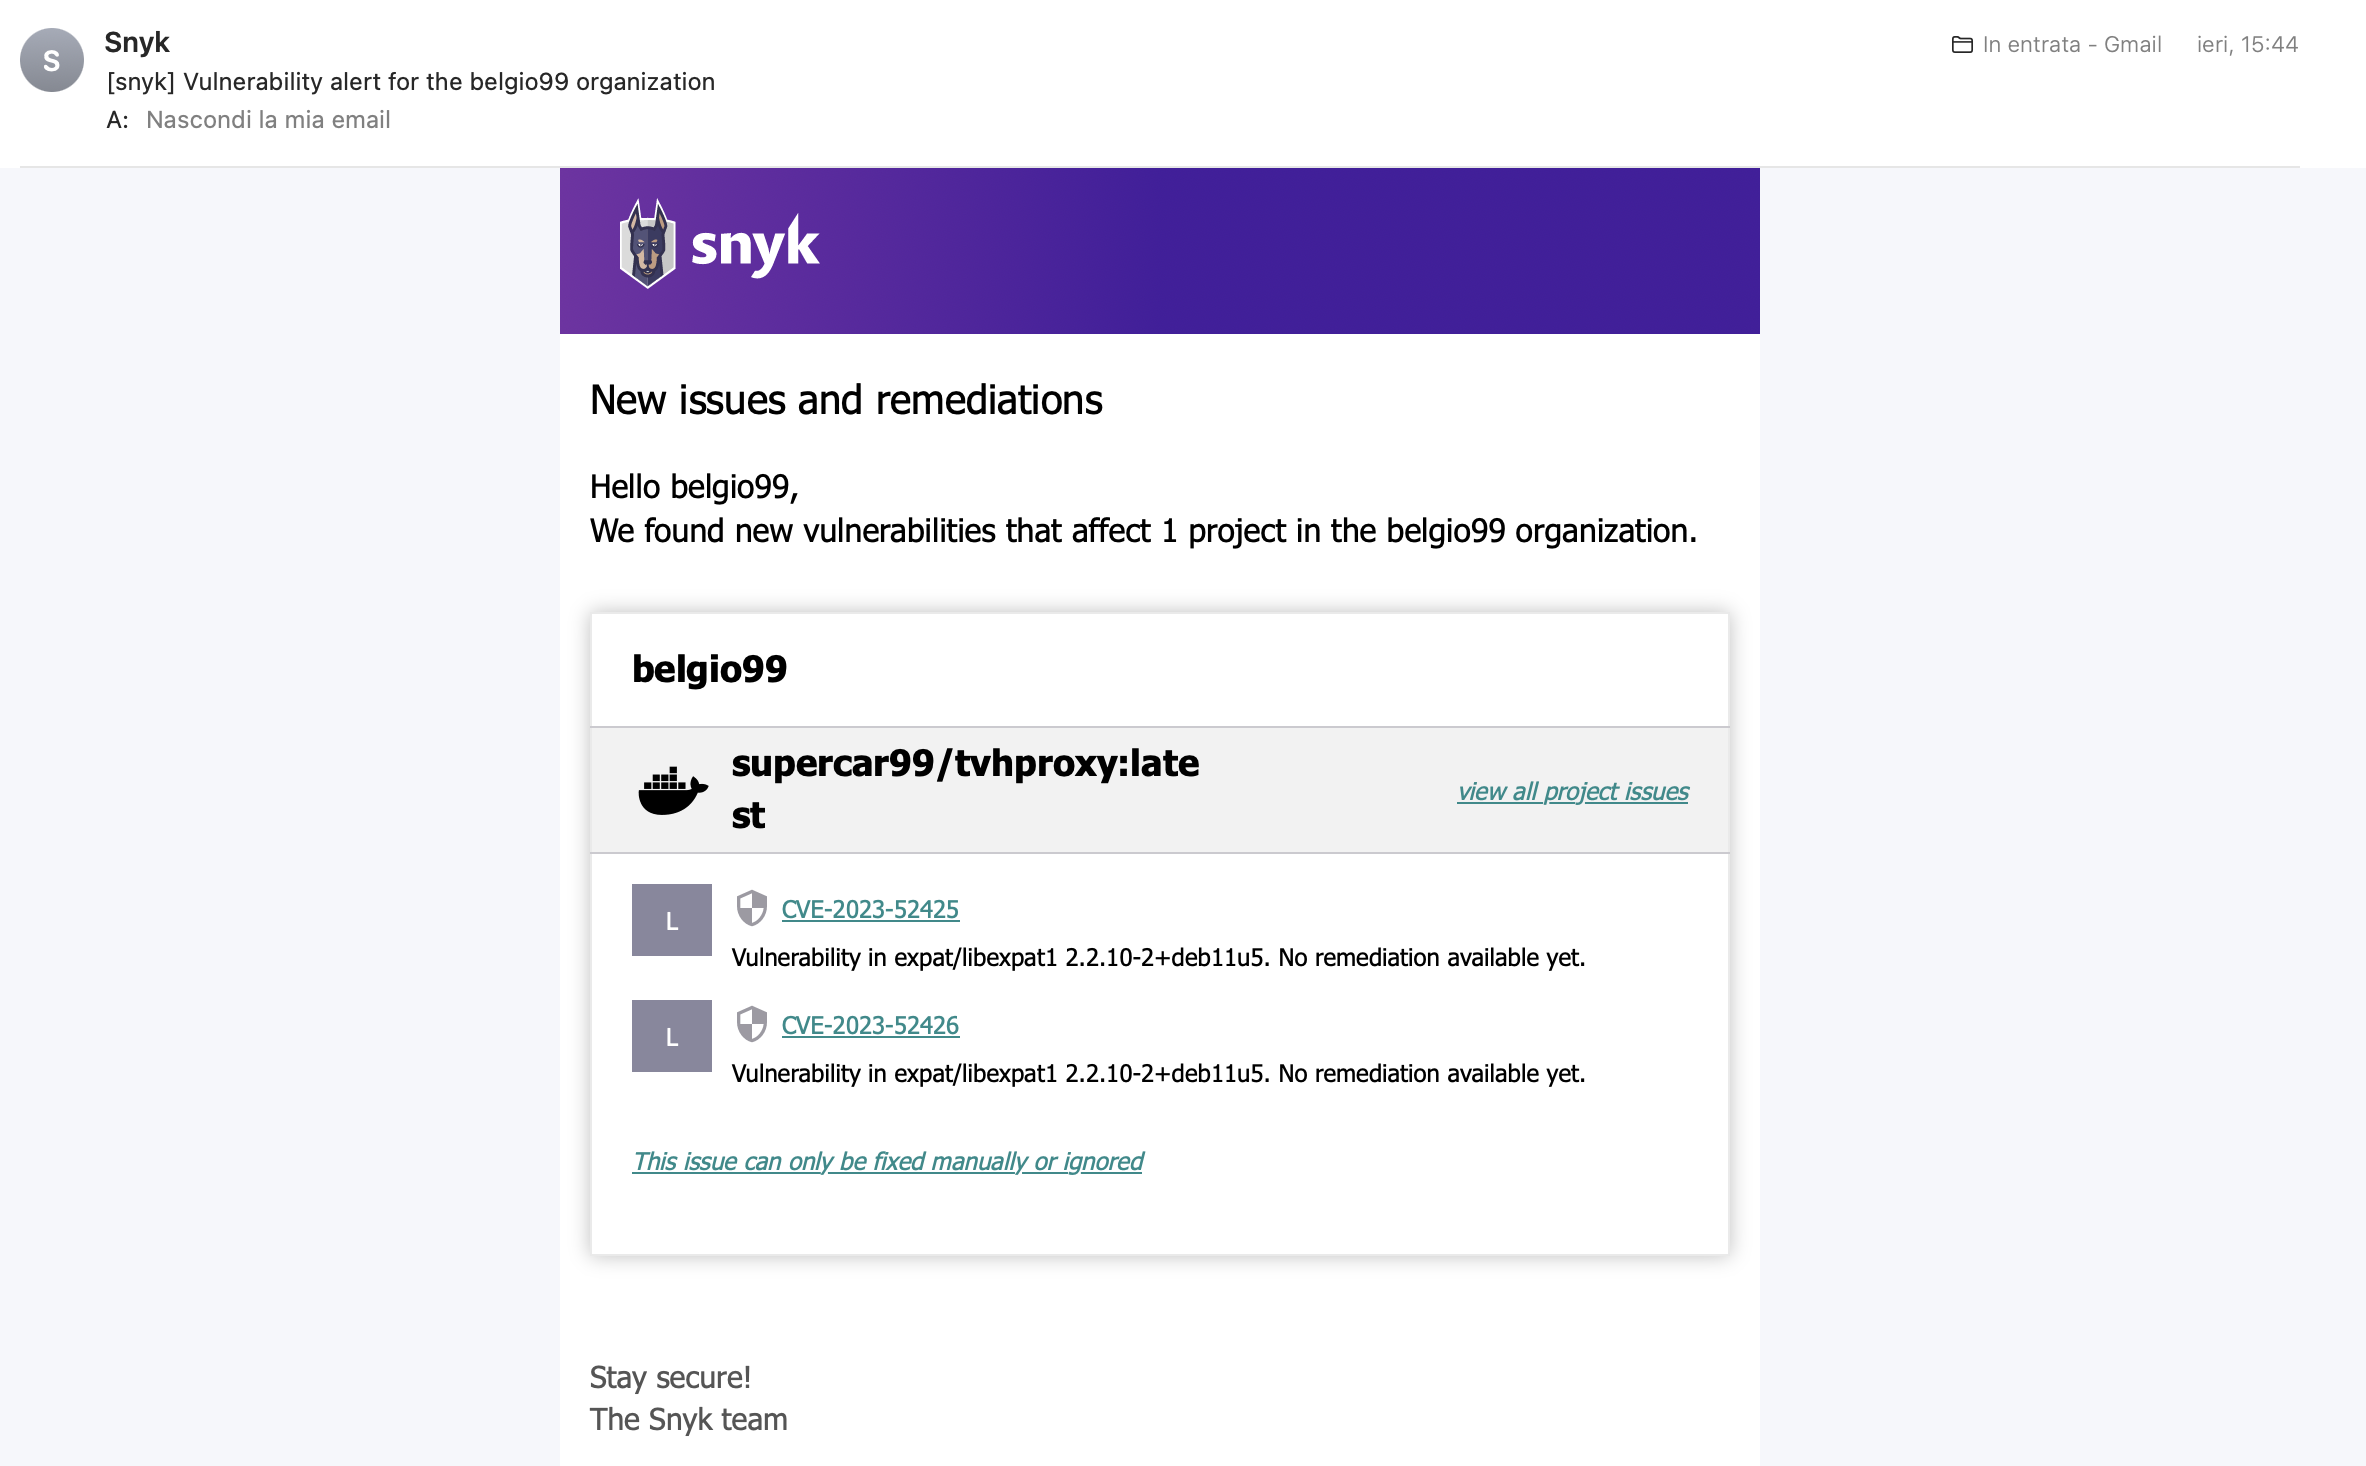
\includegraphics[width=0.8\textwidth]{immagini/capitolo2/snyk_email.png}
   \caption{E-mail ricevuta da Snyk contenente notifica di rilevazione di nuove vulnerabilità}
   \label{fig:snyk_email}
\end{figure}

Dopo la ricezione della e-mail, è stata subito eseguita una scansione con Trivy, che ha confermato la presenza delle vulnerabilità segnalate da Snyk. Questo ha permesso quindi automaticamente di verificare anche la tempestività dell'aggiornamento dei database di vulnerabilità di entrambi gli strumenti.

\subsection{Trivy: Funzionamento Offline}
Essendo un tool completamente open source, Trivy ha la capacità di poter essere utilizzato in ambienti completamente isolati, senza la necessità di connessione a Internet. Questo è possibile grazie alla possibilità di scaricare il database di vulnerabilità in locale, e di eseguire le scansioni utilizzando il database locale. Questa funzionalità è particolarmente utile in ambienti ad alta sicurezza, dove la connessione a Internet è limitata o non disponibile. Snyk, invece, richiede sempre una connessione a Internet per poter funzionare correttamente, necessitando di contattare la propria API per eseguire la vera e propria scansione.

\subsection{Snyk: Creazione Automatica di Pull Request}
Snyk offre la possibilità di creare automaticamente pull request atte a correggere le vulnerabilità rilevate. Questa funzionalità è particolarmente utile per i team di sviluppo, in quanto permette di automatizzare il processo di correzione delle vulnerabilità, riducendo il tempo e lo sforzo necessario per applicare le correzioni.

\subsection{Trivy: Scansione di Immagini VM}
Un'ultima funzione unica di Trivy è quella di poter eseguire la scansione di immagini di macchine virtuali, oltre che di immagini di container. Tramite il comando \texttt{trivy vm}, è possibile scansionare:
\begin{itemize}
   \item\textbf{File di macchine virtuali locali}: è supportata la scansione di file \texttt{.vmdk}
   \item\textbf{Cluster AWS EC2}: è supportata sia la scansione di AMI (Amazon Machine Image), sia eventuali immagini memorizzate come snapshot EBS (Elastic Block Storage).
\end{itemize}
In Figura \ref{fig:trivy_vm}, è riportato un esempio di scansione di un'immagine VM con Trivy, dove vengono rilevate varie vulnerabilità di criticità alta e media. Viene inoltre riportata in quale versione della immagine VM sono state corrette.

\begin{figure}[H]
   \centering
   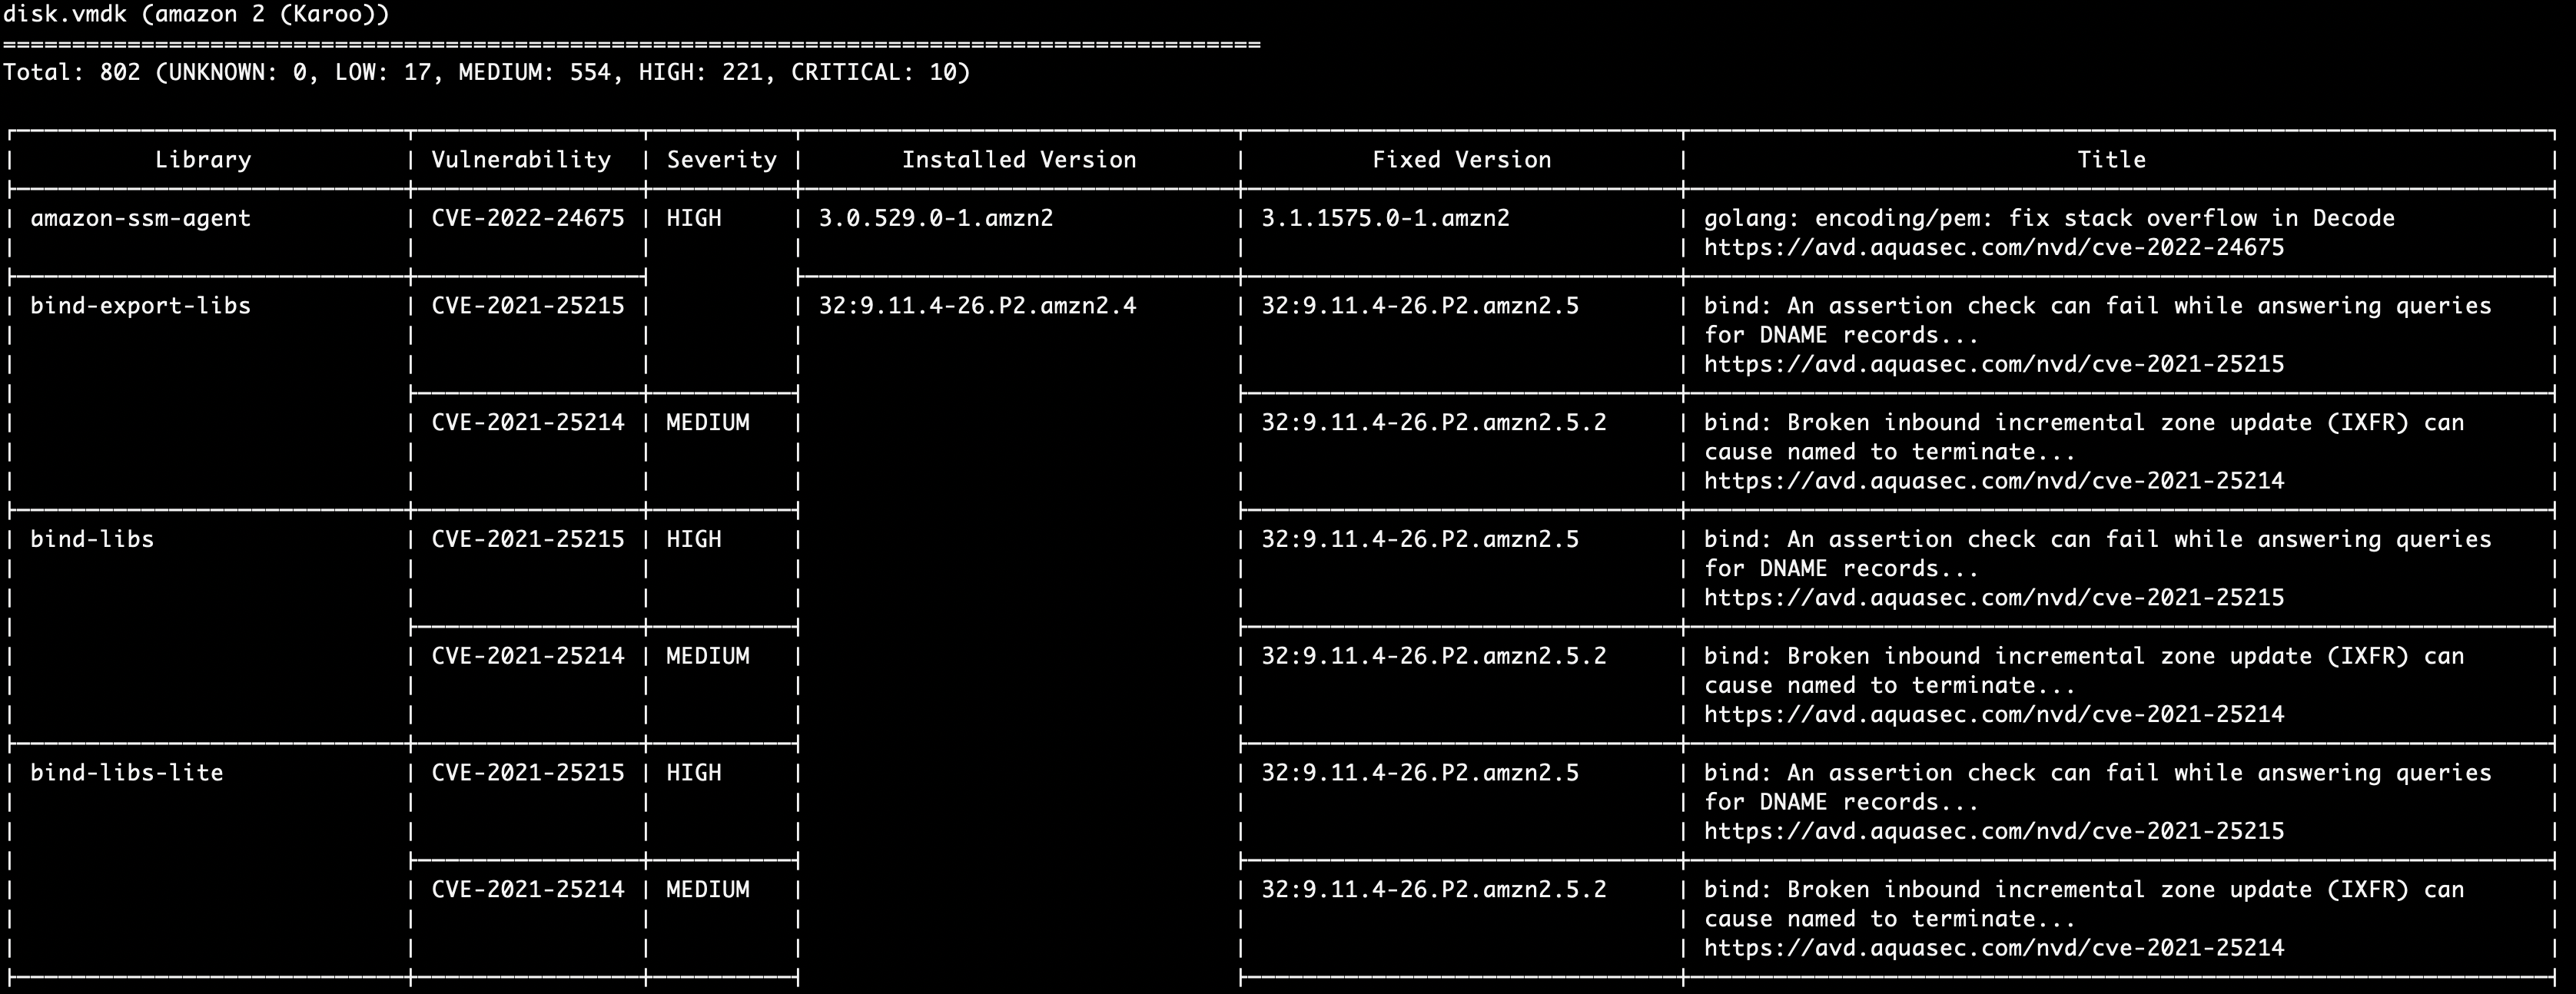
\includegraphics[width=1\textwidth]{immagini/capitolo2/trivy_vm.png}
   \caption{Esempio di scansione di un'immagine VM con Trivy}
   \label{fig:trivy_vm}
\end{figure}
Tale funzionalità rimane, al momento della stesura del presente report, come funzionalità sperimentale e ancora in sviluppo.

\section{Conclusioni}
Il confronto svolto ha evidenziato punti di forza e aree di miglioramento per entrambi gli strumenti nella gestione delle vulnerabilità software. Trivy, con la capacità di essere più sensibile per un numero maggiore di vulnerabilità, si dimostra particolarmente efficace per gli ambienti che richiedono una scansione approfondita e dettagliata, anche a costo di una maggiore incidenza di falsi positivi. La sua funzionalità di scansione di immagini VM aggiunge un ulteriore strato di utilità, rendendolo adatto per ambienti che utilizzano una varietà di soluzioni di virtualizzazione. D'altra parte, Snyk si distingue per il suo approccio conservativo nella classificazione delle vulnerabilità, potenzialmente riducendo il rischio di allarmi non necessari, e offre un valore aggiunto significativo con il suo monitoraggio continuo, assicurando che le applicazioni siano protette contro le nuove vulnerabilità non appena vengono scoperte.